%%%%%%%%%%%%%%%%%%%%%%%%%%%%%%%%%%%%%%%%%
% Journal Article
% LaTeX Template
% Version 1.3 (9/9/13)
%
% This template has been downloaded from:
% http://www.LaTeXTemplates.com
%
% Original author:
% Frits Wenneker (http://www.howtotex.com)
%
% License:
% CC BY-NC-SA 3.0 (http://creativecommons.org/licenses/by-nc-sa/3.0/)
%
%%%%%%%%%%%%%%%%%%%%%%%%%%%%%%%%%%%%%%%%%

%----------------------------------------------------------------------------------------
%	PACKAGES AND OTHER DOCUMENT CONFIGURATIONS
%----------------------------------------------------------------------------------------

\documentclass{article}

%\documentclass{aastex}  % version 5.0 or prior
%\usepackage{natbib}



\usepackage{graphicx}
\usepackage{lipsum} % Package to generate dummy text throughout this template
%\usepackage[sc]{mathpazo} % Use the Palatino font
\usepackage[T1]{fontenc} % Use 8-bit encoding that has 256 glyphs
\linespread{1.05} % Line spacing - Palatino needs more space between lines
\usepackage{microtype} % Slightly tweak font spacing for aesthetics

\usepackage[margin=1in,columnsep=20pt]{geometry} % Document margins
\usepackage{multicol} % Used for the two-column layout of the document
\usepackage[hang, small,labelfont=bf,up,textfont=it,up]{caption} % Custom captions under/above floats in tables or figures
\usepackage{booktabs} % Horizontal rules in tables
\usepackage{float} % Required for tables and figures in the multi-column environment - they need to be placed in specific locations with the [H] (e.g. \begin{table}[H])
\usepackage{hyperref} % For hyperlinks in the PDF
\usepackage{subcaption}

\usepackage{lettrine} % The lettrine is the first enlarged letter at the beginning of the text
\usepackage{paralist} % Used for the compactitem environment which makes bullet points with less space between them
\usepackage{amsmath}
\usepackage{abstract} % Allows abstract customization
\renewcommand{\abstractnamefont}{\normalfont\bfseries} % Set the "Abstract" text to bold
\renewcommand{\abstracttextfont}{\normalfont\small\itshape} % Set the abstract itself to small italic text

\usepackage{titlesec} % Allows customization of titles
%\renewcommand\thesection{\Roman{section}} % Roman numerals for the sections
%\renewcommand\thesubsection{\Roman{subsection}} % Roman numerals for subsections
%\renewcommand\thesubsubsection{\Alph{subsubsection}} % Roman numerals for subsections
\titleformat{\section}[block]{\Large\scshape}{\thesection}{1em}{} % Change the look of the section titles
\titleformat{\subsection}[block]{\large}{\thesubsection}{1em}{} % Change the look of the section titles
\titleformat{\subsubsection}[block]{}{\thesubsubsection}{1em}{} % Change the look of the section titles

\usepackage{fancyhdr} % Headers and footers
\pagestyle{fancy} % All pages have headers and footers
\fancyhead{} % Blank out the default header
\fancyfoot{} % Blank out the default footer
\fancyhead[C]{Montana State University \quad $\bullet$ \quad CSCI 466 Artificial Intelligence \quad $\bullet$ \quad Group 21} % Custom header text
\fancyfoot[RO,LE]{\thepage} % Custom footer text

\newcommand{\ve}[1]{\boldsymbol{\mathbf{#1}}}

%----------------------------------------------------------------------------------------
%	TITLE SECTION
%----------------------------------------------------------------------------------------

\title{\vspace{-15mm}\fontsize{24pt}{10pt}\selectfont\textbf{CSCI 446 Artificial Intelligence \\ Project 2 Final Report} \\[-2mm]} % Article title
\date{\today}
\author{
\large
\textsc{Roy Smart} \and \textsc{Nevin Leh} \and \textsc{Brian Marsh}\\[2mm] % Your name
}


%----------------------------------------------------------------------------------------

\begin{document}

\maketitle % Insert title

\thispagestyle{fancy} % All pages have headers and footers

%\begin{abstract}
%We present a novel way of performing MOSES data inversions using a
%\end{abstract}

%----------------------------------------------------------------------------------------
%	ARTICLE CONTENTS
%----------------------------------------------------------------------------------------

%\begin{multicols}{2} % Two-column layout throughout the main article text
\normalsize

\begin{abstract}
	Our project attempts to solve the problem of Logic and the Wumpus World by using two agents of varying sophistication to navigate the environment.
	 The agents used are a reasoning agent and a reactive agent. The reasoning agent utilized first order logic and resolution to navigate the world while the reactive agent used its current state and its previous states to make decisions. The performance of these two agents were compared to determine which one navigated the Wumpus World in the least amount of steps. It was found that the reasoning agent performed better on Wumpus Worlds of varying size, though this difference became much more apparent on Wumpus Worlds that are larger or have a large number of obstacles.
\end{abstract}
\section{Introduction}
Our task was to create a reasoning agent and reactive agent to navigate a WumpusWorld.
		\textit{Logic and the Wumpus World} is an artificial intelligence problem first proposed by Michael Genesereth, and described in detail by his student Stuart Russel\cite{ai}.  The problem involves navigating an environment known as the Wumpus World using logic to avoid dangers as the agent attempts to reach a goal.  The environment is a square grid of tiles that can be empty or contain gold for the goal state, a pit that the agent will fall into, or a monster known as a wumpus. 
		 As the agent navigates the environment, a score is calculated from the various actions that the agent makes.  
		 The objective of the game is thus to maximize the score.
		 
		 Our reasoning agent uses first order logic and the process of resolution to navigate the Wumpus World and find the gold. Resolution relies on the concept of proof by contradiction to deduce things about the Wumpus World and uses those deductions to make further deductions about the world.
		 
		 Meanwhile, our reactive agent does not use resolution and relies solely on the information supplied at its current tile and the information from tiles it has already visited to make decisions as to how to find the gold. This agent uses a kind of directed random walk to navigate the Wumpus World.
		 
		 We will be comparing the performance of the two agents to determine which one solves the Wumpus World problem more efficiently. We hypothesize that the reasoning agent will perform better than the reactive agent due to its heightened knowledge of the world and its ability to infer things about the world that the reactive agent has no way of knowing.
		 


\section{Problem Generation}
\begin{figure}
	\centering
	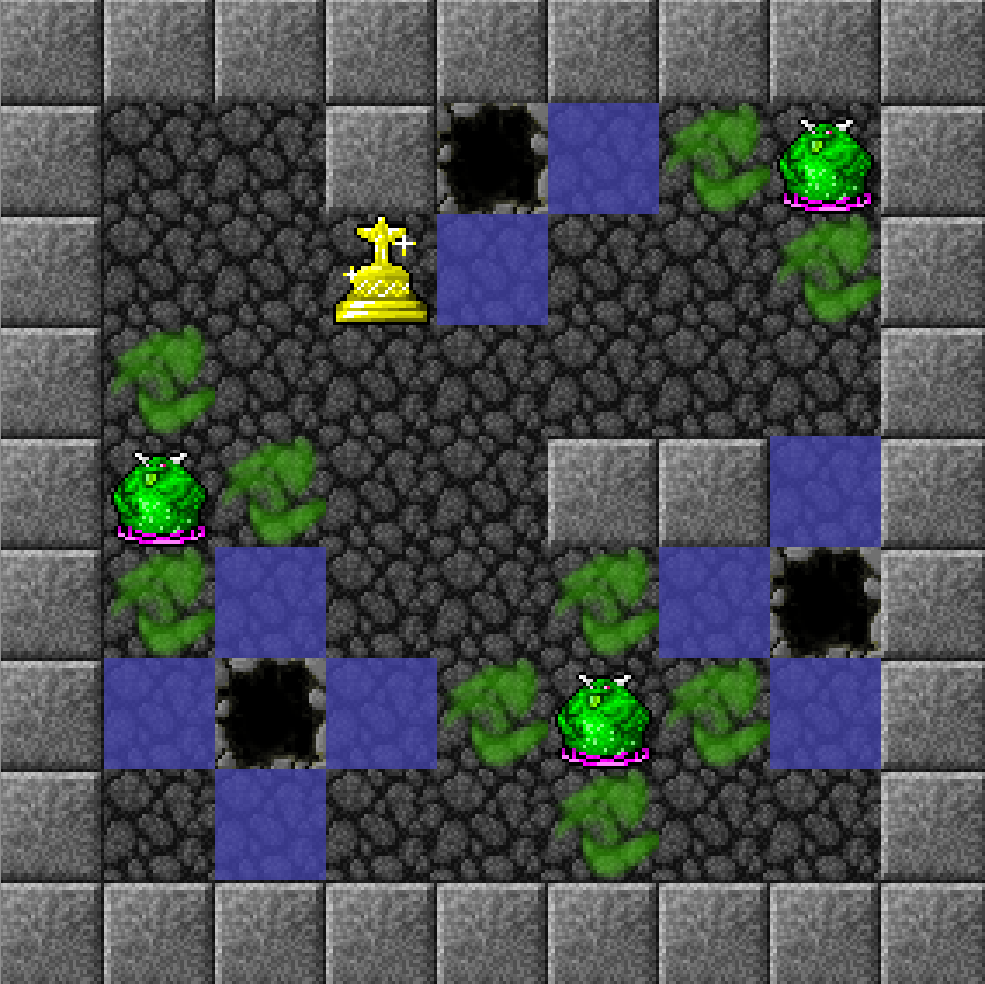
\includegraphics[width=0.5\textwidth]{images/ex_ww}
	\caption{An example of a wumpus world produced by our problem generator. The green haze represents stench and the blue tiles represent breezy squares.}
	\label{ex_ww}
\end{figure}
\section{Reactive Agent}
The first agent that was implemented was the reactive agent.
 This agent was not attached to the logical reasoning system and made decisions using an \texttt{if/else} tree.
  This agent was not a purely reactive agent as it saved old states and used that information to improve its functionality\cite{reactive}.
  

The reactive agent had very basic functionality.
 As it searched the space it would mark squares that have been visited as safe.
  If the agent encountered a breeze or a stench it would move to a randomly chosen safe tile.
   If the agent was on a tile that was not breezy and not smelly it randomly chose from the set of adjacent tiles that had not been explored yet.
    If all tiles squares had been explored a tile was chosen at random.

The reactive agent also had a special mode that was used to take chances if the space was currently searched sufficiently.
 To implement this we added a counter that incremented ever time the agent had to move to a previously explored tile and was set to zero every time the agent encountered an unexplored tile.
  If the counter reached a certain threshold a chance was taken.

\section{Reasoning Agent}
\subsection{Unification}
\subsection{Resolution}
\subsection{Pathfinding}

		

\section{Comparing Algorithm Performance}
	\label{comparisons}
	
	\subsection{Experimental Approach}
	To measure the performance of our agents we made a scoring system that decrements each time a move is made.
	 A move is defined as rotating left, rotating right, and moving forward.
	  The score will start at 1000 and finding the gold will yield an additional 1000 points to be added to the score.
	
	Using the performance measurement, we then varied the parameters of the wumpus world such as the size, number of wumpi, number of pits, etc. and plotted the relationships between the size of the world, number of obstacles, and the score.
	 For simplicities sake we used constant values for the number of pits, barriers, and wumpi.
	  Therefore, each world had the same number of pits, barriers, and wumpi. 
	  We ran each algorithm on graph sizes \{5, 10, 15,...,25\} with ten runs for each size.
	  The number of obstacles was roughly computed to have a constant obstacle density.
	
	We then used \textit{Mathematica}  to produce a 3D plot to display the data in terms of score vs. size vs. number of obstacles
	
	\subsection{Results}
		In general, the results presented exactly as hypothesized. The reasoning agent outstripped the reactive agent in terms of score regardless of the size of the world or the number of obstacles in the world. 
		However, size and the number of obstacles did affect by how much the reasoning agent was better than the reactive agent. 
		For very small board sizes with minimal obstacles the two algorithms scored almost evenly, but for large worlds with a  large number of obstacles the reasoning agent far outstrips the reactive agent.
		
		One reason the reactive agent was almost as good as the reasoning agent in small worlds is that the search space is so small that the reactive agent can search the whole safe space in nearly the same number of steps as the logical agent.
	 Since the number of steps to search the space has a large effect on the score, the scores for the small worlds are almost the same. 
		
		There are two main reasons the reasoning agent is much faster on large worlds with large amounts of obstacles.
		 The first is that the search is much better.
		  The random walk of the reactive agent gets stuck on large worlds and has a hard time searching the whole space efficiently.
		   The second reason is that the reasoning agent can reason its way through obstacles and can deduce information about tiles it has not visited yet.
		    It can also update information as more facts are reasoned out.
		     Meanwhile, the reactive agent does not have this ability and cannot mark a tile unless it has visited that tile.
	
\section{Summary}



	

	\pagebreak


	%\bibliographystyle{apj}
	\bibliographystyle{unsrt}
	
	\bibliography{sources}
\end{document}
